\documentclass{article}
\usepackage{amsmath}
\usepackage{amssymb}
\usepackage{booktabs}
\usepackage{xintexpr}
\usepackage{tikz}
\usetikzlibrary{arrows,automata}
\usepackage{float}

\newcommand{\T}{1}
\newcommand{\F}{0}
\newcommand{\TF}[1]{\if1#1\T\else\F\fi}
\newcommand{\xintTF}[1]{\xintifboolexpr{#1}{\T}{\F}}

\newcommand{\logicrule}[2]{
\begin{array}{l}
#1 \\
\midrule
\therefore #2 \\
\end{array}
}

\newcommand{\inv}[1]{#1^{-1}}

\renewcommand{\d}[1]{\,\textnormal{d}#1}
\newcommand{\dd}[2]{\frac{\d{#1}}{\d{#2}}}
\newcommand{\ddd}[2]{\dfrac{\d{#1}}{\d{#2}}}

\DeclareMathOperator{\var}{Var}
\DeclareMathOperator{\E}{\mathcal{E}}

\newcommand{\multistep}[1]{\begin{array}{rl} #1 \end{array}}
\newcommand{\subeq}{\subseteq}
\newcommand{\sub}{\subset}

\newcommand{\conj}[1]{\overline{#1}}

\setlength\parindent{0pt}
\setlength\parskip{1em}

\begin{document}

\section*{Formal Definition of Nondeterministic Finite Automata (NFA)}

This is a 5-tuple $(Q,\Sigma,\delta,q_0,F)$ where:

\begin{description}
\item[$Q$] is a finite set called the ``states''
\item[$\Sigma$] is a finite set called the ``alphabet''
\item[$\delta$]: $Q\times\{\Sigma\cup\{\epsilon\}\}\rightarrow{}P(Q)$
\item[$q_0$] is the start/initial state
\item[$F\subseteq{}Q$] is a set of accept states
\end{description}

Remember the difference between a DFA and an NFA:

\begin{description}
\item[DFA] - $\delta$: $Q\times{}\Sigma\rightarrow{}Q$
\item[NFA] - $\delta$: $Q\times\{\Sigma\cup\{\epsilon\}\}\rightarrow{}P(Q)$
\end{description}

\subsection*{Example}

\begin{figure}[H]
  \centering
  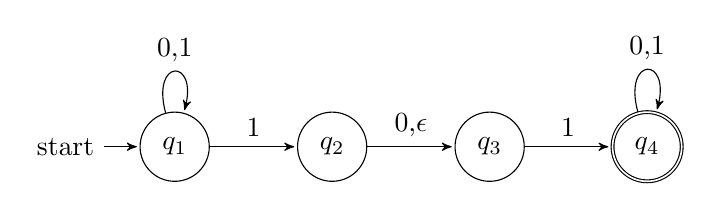
\begin{tikzpicture}[>=stealth',shorten >=1pt,auto,node distance=2cm]
    \node[initial,state] (q1)      {$q_1$};
    \node[state]         (q2) [right of=q1] {$q_2$};
    \node[state]         (q3) [right of=q2]  {$q_3$};
    \node[state,accepting] (q4) [right of=q3] {$q_4$};

    \path[->]
    (q1) edge [loop above] node {0,1} (q1)
    (q1) edge node {1} (q2)
    (q2) edge node {0,$\epsilon$} (q3)
    (q3) edge node {1} (q4)
    (q4) edge [loop above] node {0,1} (q4)
    ;
  \end{tikzpicture}
  \caption{$N_1$}
\end{figure}

The formal definition of this machine is:

\begin{description}
\item[$Q$] $=\{q_1,q_2,q_3,q_4\}$
\item[$\Sigma$] $=\{0,1\}$
\item[$\delta$]
  $\begin{array}{l|l|l|l}
  & 0 & 1 & \epsilon \\
  \midrule
  q_1 & \{q_1\} & \{q_1,q_2\} & \varnothing \\
  q_2 & \{q_3\} & \varnothing & \{q_3\} \\
  q_3 & \varnothing & \{q_4\} & \varnothing \\
  q_4 & \{q_4\} & \{q_4\} & \varnothing \\
  \end{array}$
\item[$q_1$] is the start state
\item[$F$] $=\{q_4\}$
\end{description}

We can describe this by:

$N_1$ accepts $\omega$ if we can write $\omega=y_1y_2\cdots{}y_m$
where each $y_i$ is a member of $\Sigma_\epsilon$ and there is a
sequence of states $r_0,r_1,\cdots,r_m$ exists in $Q$ with the
following 3 conditions:

\begin{enumerate}
\item $r_0=q_0$
\item $r_{i+1}\in \delta(r_i,y_{i+1}) \forall i=0,1,\cdots,m-1$
\item $r_m\in{}F$
\end{enumerate}

\subsection*{Why NFA?}

\begin{enumerate}
\item NFAs are often easier to construct than DFAs.
\item NFA might be smaller (in number of states) than DFA.
\item Computation of NFA is usually more expensive.
\item \textbf{Every} NFA can be converted to a DFA.
\end{enumerate}

\subsection*{Theorem}

Every NFA has an equivalent DFA to recognize some language.

\subsection*{Nice Application of NFAs}

We can use them to show that regular languages are closed under
regular operations (union, concatenation, star).

\textbf{Question}: Is the class of languages recognized by NFAs closed
under complementation?

\textbf{Schematic Proof}:

Take 2 regular languages $A_1$ and $A_2$. Prove that $A_1\cup{}A_2$ is
regular.

Take 2 NFAs, $N_1$ and $N_2$, and combine them into a new NFA $N$.

Suppose $N_1$ has a particular input state $q_1'$, and $N_2$ has an
input state of $q_2'$.

To combine the two machines, we could introduce a new state $q_0$
which transitions to $q_1'$ and $q_2'$ on $\epsilon$.

\begin{figure}[H]
  \centering
  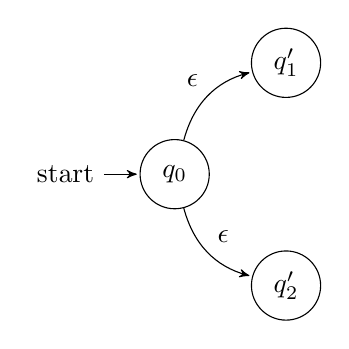
\begin{tikzpicture}[>=stealth',shorten >=1pt,auto,node distance=2cm]
    \node[initial,state] (q0) {$q_0$};
    \node[state] (q1) [above right of=q0]     {$q_1'$};
    \node[state]         (q2) [below right of=q0] {$q_2'$};

    \path[->]
    (q0) edge [bend left] node {$\epsilon$} (q1)
    (q0) edge [bend right] node {$\epsilon$} (q2)
    ;
  \end{tikzpicture}
  \caption{$N$}
\end{figure}

\subsection*{Theorem}

Class of regular languages is closed under concatenation.

\textbf{Schematic Proof}:

Given that $A_1$ and $A_2$ are regular, prove $A_1\circ{}A_2$ is
regular.

Similarly, let $N_1$ and $N_2$ be NFAs for $A_1$ and $A_2$
respectively.

If $N_1$ has, for instance, 3 end states, and $N_2$ has one input
state, then add a transition from each of the end states to the input
state of $N_2$ on $\epsilon$.

\subsection*{Theorem}

Class of regular languages is closed under the star operation.

\textbf{Schematic Proof}:

Given $A_1$ regular, prove $A_1^*$ is also regular.

Suppose we have an NFA $N_1$ for $A_1$, modify it to recognize
$A_1^*$.

Remember, the star operation means that it could have $0$ or more
instances of whatever language is recognized by the NFA.

Suppose $N_1$ has an input state $q_0$ and several final states
$f_0,f_1$.

Add a new state as the input state $q_0'$. Map $q_0'$ to $q_0$ on
$\epsilon$. Map each of $f_0,f_1$ to $q_0'$ on $\epsilon$.

\section*{Equivalence of NFA and DFA}

Let $N=(Q,\Sigma,\delta,q_0,F)$ be the NFA recognizing the language
$A$. We want to construct the DFA $M=(Q',\Sigma,\delta',q_0',F')$ to
recognize $A$.

First, we want to consider the case when $N$ has no $\epsilon$
transitions.

\textbf{Notation}: For any $R\subseteq{}Q$, define $E(R)$ to be the
collection of states that can be reched from $R$ by going only along
$\epsilon$ transitions, including members of $R$ themselves.

\[
E(R)=R\cup\left\{q\in{}Q\middle|\forall 1\le{}i\le{}k(\exists{}r_i\in{}R),\quad r_{i+1}\in\delta(r_i,\epsilon),\quad r_k=q\right\}
\]

We want to modify $\delta$ of $M$ to place additional links/edges on
all states that can be reached by going along $\epsilon$ edges after
every step.

For $R\in{}Q'$ and a symbol $a\in\Sigma$, let $\delta'(R,a)$ be:

\[
\delta'(R,a)=\left\{q\in{}Q\middle|q\in\delta(r,a)\text{ for some }r\in{}R\right\}
\]

For the original NFA, replace $\delta(r,a)$ with $E(\delta(r,a))$.

Ultimately, we want

\[
\delta'(R,a)=\{q\in{}Q|q\in E(\delta(r,a))\text{ for some}r\in{}R\}
\]

Our machine can then be given as:
$M=(Q',\Sigma,\delta',q_0',F')$. Where $q_0'$... yolo

\subsection*{Example}

\begin{figure}[H]
  \centering
  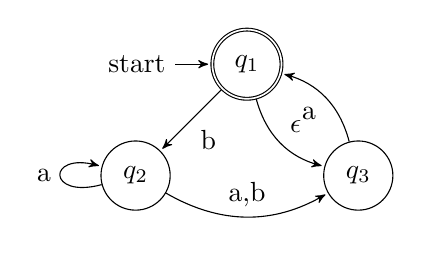
\begin{tikzpicture}[>=stealth',shorten >=1pt,auto,node distance=2cm]
    \node[initial,state,accepting] (q1) {$q_1$};
    \node[state] [below left of=q1] (q2) {$q_2$};
    \node[state] [below right of=q1] (q3) {$q_3$};

    \path[->]
    (q1) edge node {b} (q2)
    (q1) edge [bend right] node {$\epsilon$} (q3)
    (q2) edge [loop left] node {a} (q2)
    (q2) edge [bend right] node {a,b} (q3)
    (q3) edge [bend right] node {a} (q1)
    ;
  \end{tikzpicture}
  \caption{$N_4$}
\end{figure}

Note that $N_4$ is described by $N_4=(Q,\Sigma,\delta,q_1,F)$ where:

\begin{description}
\item[$Q$]: $\{1,2,3\}$ with $i$ for $q_i$
\item[$\Sigma$]: $\{a,b\}$
\item[$q_1$]: $1$
\item[$F$]: $\{1\}$
\end{description}

$N_4$ has 3 states means we have 2 subsets of states (power set).

Let $D$ be the DFA we seek so that:

\[
Q'=P(Q)=\{\varnothing,\{1\},\{2\},\{3\},\{1,2\},\{1,3\},\{2,3\},\{1,2,3\}\}
\]

The start state for $D$ is in $E(\{1\})=\{1,3\}=q_0'$. Note that this
is not 2 states. This will become 1 state in the DFA.

Now we look at $F'=\{\{1\},\{1,2\},\{1,3\},\{1,2,3\}\}$. Note that
each of these has a $1$ in them, for the end state ($q_1$).

\end{document}
